% !TeX spellcheck = de_DE
\section{Optimierungsprobleme}
\label{sec:analysis_optimzation_problems}
Nach erfolgreicher Verifizierung der Funktionalität wird in diesem Kapitel auf verschiedene andere Optimierungsprobleme eingegangen, anhand derer die Analyse durchgeführt werden soll. Grundsätzlich ist bei der Implementierung zu beachten, dass keine zu aufwändigen Optimierungsprobleme verwendet werden, da der Raspberry Pi 4 grundsätzlich nicht so leistungsfähig ist und die benötigte Optimierungszeit sehr hoch sein kann. Daher werden im folgenden hauptsächlich klassische Probleme des bestärkenden Lernens aus dem OpenAI Gym verwendet. Die ausgewählten Umgebungen sind das \emph{Cartpole}, \emph{MountainCar} und das \emph{Pendulum} Problem. Im Folgenden wird auf die entsprechenden Optimierungsprobleme genauer eingegangen und die Implementierung der Fitnessfunktion und Abbruchbedingung kurz vorgestellt. 

\subsection{Cartpole}
Die \emph{Cartpole} Umgebung, auch als \emph{Pole Balancing} bezeichnet, wurde bereits 1983 das erste mal in Quelle \cite{barto1983neuronlike} vorgestellt und ist auch heute noch ein bekanntes Optimierungsproblem, welches in vielen Publikationen verwendet wird. Auch im OpenAI Gym ist dieses Problem entsprechend der Beschreibung aus Quelle \cite{barto1983neuronlike} enthalten und in Abbildung \ref{fig:cartpole_environment} dargestellt. In der Umgebung befinden sich zwei Gegenstände. Das erste ist ein Waagen, welcher von dem Agenten nach links und rechts bewegt werden kann. Hierauf befindet sich ein Balken, welcher am unteren Ende mit dem Waagen verbunden ist. Entsprechend seiner Position, kann dieser nach links oder rechts kippen. Das Ziel für den Agenten ist, durch Steuerung des Wagens den Balken so lange wie möglich senkrecht zu balancieren. Bezüglich der Abbruchbedingung gilt, dass der Agent scheitert wenn der Balken entweder mehr als $15\degree$ auf eine Seite kippt oder wenn der Wagen sich zu weit vom Zentrum entfernt hat. Als Eingabewerte für das \ac{KNN} werden von der Umgebung vier Werte zur Verfügung gestellt, für welche je ein Eingabeneuron erstellt wird. Dies ist unter anderem die Position und Geschwindigkeit des Wagens, der aktuelle Winkel des Balkens und dessen Änderungsrate. Zusätzlich besitzt das erstellte \ac{KNN} zwei Ausgabeneuronen, welche die jeweilige Richtung repräsentieren. Ist der Aktivierungsgrad des erstens \emph{Output}-Neurons höher als der des zweiten, wird der Wagen nach links bewegt und andernfalls nach rechts.
\begin{figure}[!h]
	\centering
	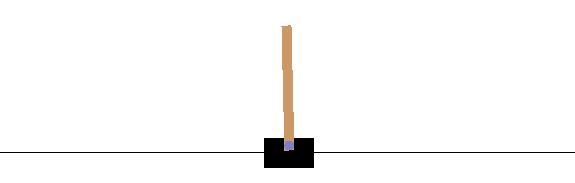
\includegraphics[width=0.5\textwidth]{./img/cartpole_env.JPG} 
	\caption{Darstellung der \emph{Cartpole} Umgebung}
	\label{fig:cartpole_environment}
\end{figure} 
Bevor die Evaluation mit dieser Umgebung durchgeführt wird, müssen noch die Fitnessfunktion, Lösungsbedingung und Konfiguration festgelegt werden. Beim klassischen bestärkenden Lernen, wie es in Kapitel \ref{subsubsec:reinforcment_learning} beschrieben ist, erhält der Agent nach jedem Zeitschritt einen \emph{reward}. Da das OpenAI Gym primär für diese Art des Lernens konzipiert ist, wird auch hier nach jeder Aktion in der Umgebung ein \emph{reward} zurück gegeben. In diesem Fall erhält ein Agent bis er scheitert für jeden Zeitschritt einen \emph{reward} mit der Wertigkeit $1$. Mit diesen muss für neuroevolutionäre Algorithmen eine Fitnessfunktion definiert werden. In diesem Beispiel ist das Vorgehen einfach. Der Fitnesswert wird berechnet indem die erhaltenen \emph{rewards} aggregiert und der erhaltene Wert am Ende der Evaluation quadriert wird. Somit soll wie zuvor beim XOR-Problem besseren Agenten ein proportional höherer Fitnesswert zugewiesen werden. Das Optimierungsverfahren wird abgebrochen, wenn ein Agent den Balken für mindestens 500 Zeitschritte balancieren kann. Die restlichen Parameter wurden aus dem vorherigen Beispiel übernommen und nicht wieder geändert.
\begin{figure}[!h]
	\centering
	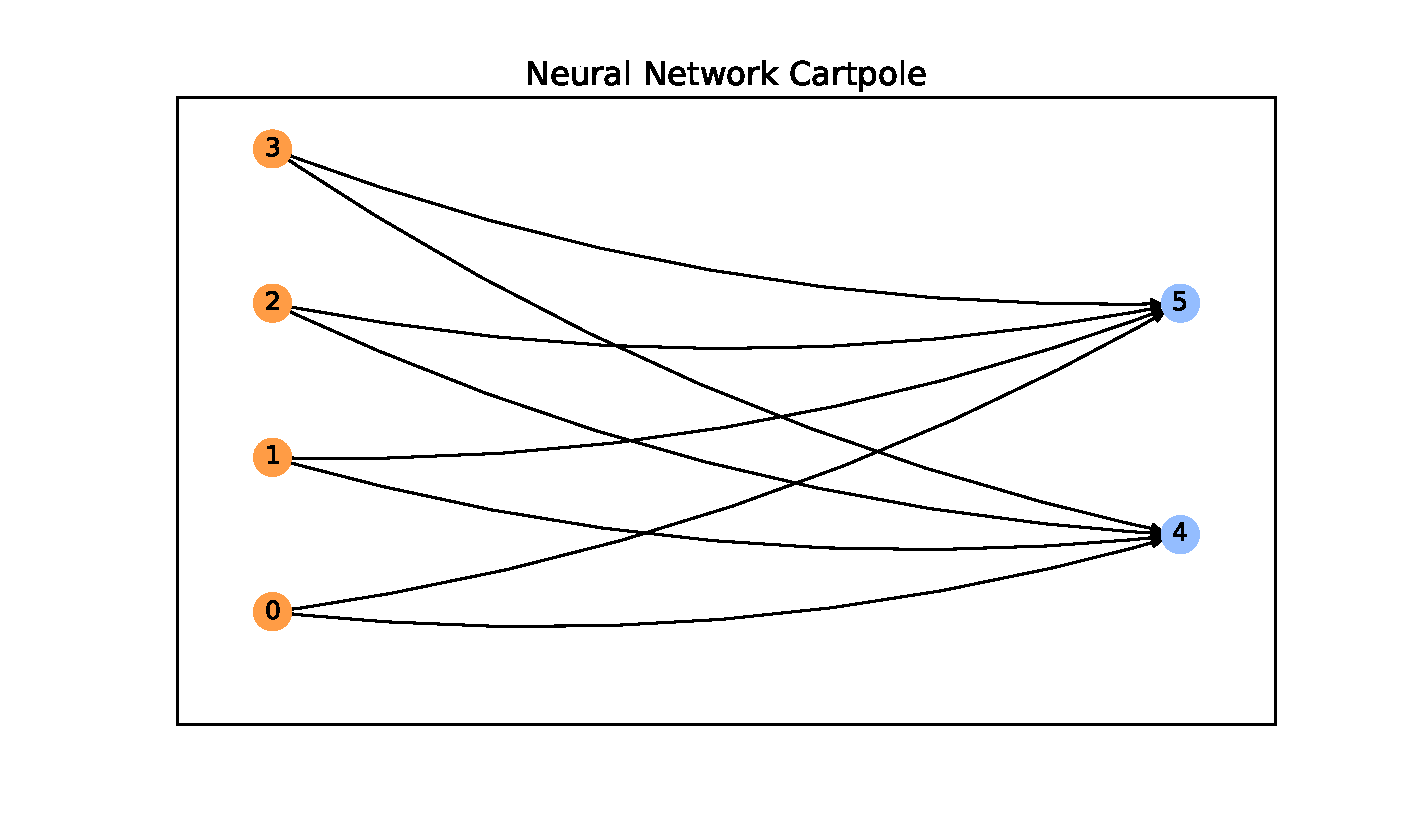
\includegraphics[width=0.7\textwidth]{./img/pole_balancing_single_core/cartpole_neuroal_network.pdf} 
	\caption{Struktur des finalen \ac{KNN} im \emph{Cartpole} Optimierungsproblem}
	\label{fig:cartpole_neural_network}
\end{figure}
\\\\
Allerdings stellt sich beim Ausführen dieses Optimierungsproblems heraus, dass es für die Analyse ungeeignet ist. Bereits in der initialen Population, für welche die Agenten zufällig erstellt werden, sind \ac{KNN} vorhanden, die die Abbruchbedingung erfüllen und das Optimierungsproblem lösen. Ein solches ist in Abbildung \ref{fig:cartpole_neural_network} dargestellt. Wie die anderen \ac{KNN} in der initialen Population, besitzt auch dieses keine \emph{Hidden}-Neuronen und zeigt, dass für das Lösen dieses Optimierungsproblem keine komplexen Entscheidungen notwendig sind. Es ist beispielsweise mit dem Winkel des Balken möglich auf die auszuführende Aktion zu schließen. Neigt sich der Balken nach rechts, bewegt sich der Wagen in diese Richtung und umgekehrt. Dies ist einer der Gründe warum dieses Optimierungsproblem im weiteren Verlauf der Arbeit nicht weiter verwendet wird. Ein weiterer Grund ist, dass durch die Fehlende Optimierung keine Ausführungszeiten über mehrere Generationen gemessen werden können, welche eine notwendige Grundlage für den späteren Vergleich sind.

\subsection{Mountain Car}

\subsection{Pendulum}


